
%----------------------------------------------------------------------------------------
%	PACKAGES AND THEMES
    %----------------------------------------------------------------------------------------
    \documentclass[aspectratio=169,xcolor=dvipsnames]{beamer}
    \usetheme{SimplePlus}
    \usecolortheme{default}
    \definecolor{grayedout}{RGB}{200,200,220}  % Choose whichever optiox`n you prefer

    % \pdfcompresslevel=0
    % \pdfobjcompresslevel=0

    \usepackage{threeparttable}
    \usepackage{hyperref}
    \usepackage{subfig}
    \usepackage{bbm}
    \usepackage{graphicx} % Allows including images
    \usepackage{booktabs} % Allows the use of \toprule, \midrule and \bottomrule in tables
    \usepackage{tikz}
    \usepackage{appendixnumberbeamer}
    \usepackage{graphicx}
    \usepackage{animate}
    \usepackage{multimedia}
    \usepackage{adjustbox}

    \graphicspath{{../../stata/figures/}}

    \usepackage[T1]{fontenc}
    \usepackage{lmodern}


    %----------------------------------------------------------------------------------------
    %	CITATIONS
    %----------------------------------------------------------------------------------------
    \usepackage[natbibapa]{apacite}
    \makeatletter
    \NAT@longnamesfalse
    \makeatother
    %----------------------------------------------------------------------------------------
    %	BULLET POINTS
    %----------------------------------------------------------------------------------------

    \setbeamertemplate{itemize item}{\color{structure!100}\scriptsize\raise1.25pt\hbox{\donotcoloroutermaths$\circ$}}
    \setbeamertemplate{itemize subitem}{\color{structure!100}\scriptsize\raise1.25pt\hbox{\donotcoloroutermaths$\circ$}}

    %----------------------------------------------------------------------------------------
    %	TRANSITION PAGE
    %----------------------------------------------------------------------------------------

    \setbeamercovered{transparent}
    \renewcommand{\footnotesize}{\fontsize{8pt}{11pt}\selectfont}

    \AtBeginSection[] {
        \begingroup
        \setbeamertemplate{background}{
          
\begin{tikzpicture}
          \useasboundingbox (0,0) rectangle (\paperwidth,\paperheight);
          \fill[color=DarkBlue] (0,0) rectangle (\paperwidth,\paperheight);
          % If you have a background image:
          % \node at (current page.center) {\includegraphics[width=\paperwidth,height=\paperheight]{background.jpg}};
          \end{tikzpicture}
        }
        \begin{frame}[plain]
          \vspace*{\fill}
          \centering
          \usebeamerfont{section title}
          \usebeamercolor[fg]{section title}
          \color{white}\huge\insertsection
          \vspace*{\fill}
        \end{frame}
        \endgroup
      }

    %----------------------------------------------------------------------------------------
    %	TITLE PAGE
    %----------------------------------------------------------------------------------------

\title[short title]{Does Autoplay Drive Excessive Screen Time? Evidence from an Online experiment} % The short title appears at the bottom of every slide, the full title is only on the title pages
    \subtitle{1-hour presentation}

    \date{25 November 2025} % Date, can be changed to a custom date

    \author[shortname]{Reha Tuncer}
    
    \institute[shortinst]{University of Luxembourg \newline Faculty of Law, Economics, and Finance (FDEF)}
    
    

    %----------------------------------------------------------------------------------------
    %	PRESENTATION SLIDES
    %----------------------------------------------------------------------------------------

\begin{document}

\begin{frame}
  % Print the title page as the first slide
  \titlepage
  \hideprogressbar
\end{frame}
% today i am going to talk about autoplay. this is a design feature I am sure everyone in this room who was ever used youtube or facebook has seen. autoplay is about how video content is delivered to online users and has been a daily part of our lives for a couple of years now. for example you land on a website and all of a sudden there is an ad that starts playing. you finish an episode of a tv series on netflix and the next episode starts without you clicking something. or perhaps you watched a video on facebook and the next one automatically scrolls in your screen and once again, starts playing. oftentimes, this sudden stimulus captures our attention immediately. sometimes, after getting exposed to this stimulus, we may even forget why we opened the app in the first place :) 

% our online experience across many platforms was not like this a couple of years ago. to inrcease the time spent on their platforms, companies continously test new ways of capturing user attention and making users consume content for longer periods of time. there are two ways that companies can do this. First, companies have propriatary recommendation algorithms that 'feed' users the content that they may like, and second companies can design -much like architects- the digital environmants in which content consumption takes place. 

% companies are running the type of the experiment i will present today continously to optimize their platforms. with advancing technologies and better network access, its no wonder that we ended up in a situation where content is delivered as soon as it can be loaded from servers. the question is what are the effects of autoplayed content? 

%  my focus today is on the design aspect. i will present an online laboratory experiment where I control for the algorithmic content curation, and thereby isolating the effect of autoplaying videos on content consumption. 
\begin{frame}{Motivation}
  \showprogressbar
  \centering
  \animategraphics[loop, width=6cm]{10}{nyt_autoplay-}{0}{134}
  \vspace{0.5em}
  \begin{itemize}
    \item Autoplay is a ubiquitous design feature delivering video content without explicit consent
    \item It is a product of the extensive A/B testing done by companies to increase engagement
          % \item Autoplay delivers content automatically across platforms (YouTube, Netflix, Facebook)
          % \item Companies maximize screen time via: (1) recommendation algorithms, (2) interface design
          % \item Despite widespread use, causal effects of autoplay remain unclear
          % \item This study: Laboratory experiment isolating autoplay's effect by controlling content algorithms
  \end{itemize}
\end{frame}

\begin{frame}{Motivation}
  \begin{itemize} %[<+->]
    \item Companies maximize content consumption via (1) proprietary recommendation algorithms, (2) interface design
    \item Despite subsequent legislative action in US \href{https://www.congress.gov/bill/116th-congress/senate-bill/2314/text}{(SMART Act of 2019)} and in EU \href{https://digitalfairnessact.com/what-is-the-digital-fairness-act}{(Digital Fairness Act)}, causal effects of autoplay remain unclear
    \item In order to inform policy, welfare implications of interface design needs deeper study
    \item This study is an (online) laboratory experiment isolating autoplay's effect on content consumption
  \end{itemize}
\end{frame}

\begin{frame}{Research Question}
  \begin{itemize} %[<+->]
    \item Does autoplay, in isolation from algorithmic content curation, increase video consumption and override users' stated preferences?
  \end{itemize}
\end{frame}

%  mention papers at least 1 of 4 --> credibility

\begin{frame}{Related Literature}
  \begin{enumerate}
    \item Digital addiction and welfare effects of social media
          \begin{itemize}
            \item \citet{allcott2020welfare, allcott2022digital, braghieri2022aer, bursztyn2023}
          \end{itemize}
    \item Intertemporal choice and self-control
          \begin{itemize}
            \item \citet{ericson2019intertemporal, houser2018gaeb, bonein2015self, ek2023too}
          \end{itemize}
    \item Interface design and user agency
          \begin{itemize}
            \item \citet{mathur2021p2cchfcs, lyngs2020p2cchfcs, lukoff2021design,schaffner2023pahia, purohit2023starving}
          \end{itemize}
    \item Field evidence on autoplay
          \begin{itemize}
            \item \citet{hiniker2018coco, schaffner2025pahi}
          \end{itemize}
  \end{enumerate}
\end{frame}

\begin{frame}{Contribution}
  \begin{enumerate} %[<+->]
    \item Main: First study to causally identify autoplay's effect on content consumption
    \item Methodological: Intertemporal choice with real-time labor-leisure tradeoff
    \item Policy: Lessons for regulation
  \end{enumerate}
\end{frame}

\begin{frame}{Theoretical Framework}
  \begin{itemize} %[<+->]
    \item Temptation in digital context, as in \citet{kleinberg2022challenge}
    \item Preregistered Hypotheses (\url{https://osf.io/mfkbc/overview})
          \begin{enumerate}
            \item Autoplay increases video consumption
            \item Autoplay causes more preference reversals
            \item Participants demand commitment against autoplay
          \end{enumerate}
  \end{itemize}
\end{frame}

% slide about preview results

\begin{frame}{Preview of Results}
  \begin{itemize}
    \item Autoplay shows no causal effect on video consumption when content is held constant
    \item Participants exhibit positive Willingness To Pay (WTP) for autoplay (6.72 pence/hour), viewing it as a convenience feature rather than a self-control problem
  \end{itemize}
\end{frame}

\begin{frame}{Experimental Design Overview}
  \begin{table}
    \centering
    \footnotesize
    \begin{threeparttable}
      \begin{tabular*}{0.7\columnwidth}{@{\extracolsep{\fill}}l c@{}}
        \toprule
        & \textbf{Timeline}  \\
        \midrule
        Block 1 & Practice $\rightarrow$ Time Choice $\rightarrow$ Main Session \\
        Block 2 & Practice $\rightarrow$ Multiple Price List $\rightarrow$ Time Choice $\rightarrow$ Main Session \\
        \bottomrule
      \end{tabular*}
      \label{tab:overview}
    \end{threeparttable}
  \end{table}
  \vspace{2em}  % Add some space to align better with the table
  \begin{itemize}
    \item Two separate data collections with separate samples (Blocks 1 \& 2)
    \item Objective: Time allocation across a labor and a leisure task
    \item 2-minute Practice Session to familiarize with tasks
    \item Time Choice: a hyphotetical time allocation decision
    \item Main session: 20 minutes of time to be spent between tasks
    \item Block 2: Multiple Price List (MPL) to elicit WTP for autoplay
  \end{itemize}
\end{frame}

\begin{frame}{Transcription Task}
  \begin{columns}[T]
    \begin{column}{0.38\textwidth}
      \begin{itemize} %[<+->]
        \item Retype randomly generated CAPTCHAs (35 characters, blurred and distorted)
        \item Payment at 0.15 pence/second
        \item Quality requirements at 70\% accuracy, minimum 1 submission/minute
        \item Average time 41 seconds per CAPTCHA
      \end{itemize}
    \end{column}
    \begin{column}{0.62\textwidth}
      \centering
      
\includegraphics[width=0.65\columnwidth]{typing.png}
    \end{column}
  \end{columns}
\end{frame}

\begin{frame}{Watching Task}
  \begin{columns}[T]
    \begin{column}{0.38\textwidth}
      \begin{itemize} %[<+->]
        \item Watch funny animal videos curated from YouTube and TikTok
        \item Payment at 0.10 pence/second
        \item 80 videos total, short duration (mean 12.25 sec.)
        \item Videos rated positively (median 7/10)
      \end{itemize}
    \end{column}
    \begin{column}{0.62\textwidth}
      \centering
      
\includegraphics[width=0.575\columnwidth]{watching.png}
    \end{column}
  \end{columns}
\end{frame}

\begin{frame}{Treatment Variation}
  \begin{table}
    \centering
    \footnotesize
    \begin{threeparttable}
      \begin{tabular*}{0.9\columnwidth}{@{\extracolsep{\fill}}lc c@{}}
        \toprule
        & \multicolumn{1}{c}{\textbf{Autoplay}} & \multicolumn{1}{c}{\textbf{Control}}  \\
        \midrule
        Playback & Videos play continuously & Participants click to play each video \\
        Transition & Automatic scrolling to next video & Next video visible but requires click \\
        \bottomrule
      \end{tabular*}
      \label{tab:treatment}
    \end{threeparttable}
  \end{table}
  \vspace{2em}
  \begin{itemize}
    \item Identical videos and playlist order
    \item Same tab structure, progress bar, and timer
    \item Not possible to skip videos (controls disabled)
    \item Randomization occurs before Practice session
  \end{itemize}
\end{frame}

\begin{frame}{Multiple Price List}
  \begin{columns}[T]
    \begin{column}{0.38\textwidth}
      \begin{itemize} %[<+->]
        \item Only in Block 2
        \item 9 binary decisions
        \item Allows probabilistically selecting into treatment or control
        \item Bonus earnings range between 0.5 and 0.05 pounds
        \item 1 out of 9 choices implemented at random
      \end{itemize}
    \end{column}
    \begin{column}{0.62\textwidth}
      \centering
      
\includegraphics[width=0.4\columnwidth]{mpl.png}
    \end{column}
  \end{columns}
\end{frame}

\begin{frame}{Time Choice}
  \begin{columns}[T]
    \begin{column}{0.38\textwidth}
      \begin{itemize} %[<+->]
        \item Two-day online experiment
        \item 24-hour cooling off period to measure planned vs. actual behavior
        \item Real-time feedback on expected earnings with slider tool (20-second increments)
        \item Corner solutions allowed (0\% or 100\% on either task) with max. earnings difference at 0.6 pounds
        \item 5\% of choices randomly made binding for Day 2
      \end{itemize}
    \end{column}
    \begin{column}{0.62\textwidth}
      \centering
      
\includegraphics[width=0.7\columnwidth]{time-choice.png}
    \end{column}
  \end{columns}
\end{frame}

\begin{frame}{Experimental Design Recap}
  \begin{columns}[T]  % T option aligns the top of the columns
    \begin{column}{0.38\textwidth}  % Left column for placeholder text
      \begin{itemize}
        \item Key tradeoff: higher earnings from Transcription vs. lower effort from Watching
        \item Elicit informed time allocation preferences before actualization to measure preference reversals in any direction
        \item Treatment only changes the autoplay setting in Watching task
      \end{itemize}
    \end{column}
    \begin{column}{0.62\textwidth}  % Right column for the table
      \begin{table}
        \centering
        \footnotesize
        \begin{threeparttable}
          \begin{tabular*}{0.9\columnwidth}{@{\extracolsep{\fill}}lc c@{}}
            \toprule
            & \multicolumn{1}{c}{\textbf{Day 1}} & \multicolumn{1}{c}{\textbf{Day 2}}  \\
            \midrule
            Block 1 & Practice $\rightarrow$ Time Choice & Main Session \\
            Block 2 & Practice $\rightarrow$ MPL $\rightarrow$ Time Choice & Main Session \\
            \bottomrule
          \end{tabular*}
          \label{tab:recap}
        \end{threeparttable}
      \end{table}
    \end{column}
  \end{columns}
\end{frame}

\begin{frame}{Procedures}
  \begin{itemize}
    \item Prolific participant pool (online platform for academic research)
    \item Adult British residents, fluent in English
    \item Sampling based on preregistered power calculations (\url{https://osf.io/mfkbc/overview})
    \item 276/301 participants completed Block 1 (92\% response rate)
    \item 57/60 participants completed Block 2 (95\% response rate)
    \item Fixed fee: £2.75 upon completion
    \item Average total earnings: £4.08
    \item Average total time spent: 30 minutes
  \end{itemize}
\end{frame}

\begin{frame}{Internal Controls}
  \begin{columns}[T]  % T option aligns the top of the columns
    \begin{column}{0.6\textwidth}  % Left column for placeholder text
      \begin{itemize}
        \item 2 attention checks
        \item Desktop only, Chromium browsers on both days
        \item Minimum internet speed >30 Mbps on both days
        \item Real-time mouse monitoring using JavaScript
        \item Post-experiment validation (self-reported honesty and network quality)
        \item Exclusion criteria: Connection issues (6\%), honesty (9\%), mouse monitoring (15\%)
      \end{itemize}
    \end{column}
    \begin{column}{0.4\textwidth}  % Right column for the table
      \centering
      \begin{figure}
        \includegraphics[width=0.7\columnwidth]{qr.png}
        \caption{Experience Day 1 as a visitor!}
      \end{figure}
    \end{column}
  \end{columns}
\end{frame}

\begin{frame}{Balance table Block 1}
  \begin{table}
    \begin{adjustbox}{width=0.9\textwidth, totalheight=\textheight-4\baselineskip,keepaspectratio}
      \centering
      \begin{threeparttable}
        \begin{tabular*}{\textwidth}{@{\extracolsep{\fill}}lcc c@{}}
          \toprule
          & \multicolumn{1}{c}{Autoplay} & \multicolumn{1}{c}{Control} & \multicolumn{1}{c}{\textit{p}} \\
          & \multicolumn{1}{c}{N = 79} & \multicolumn{1}{c}{N = 105} & [A = C]\\
          \midrule
          \textit{\textbf{Gender}} & & & \\
          Female & 36 (45.57\%) & 53 (50.48\%) & 0.510 \\ \midrule
          \textit{\textbf{Age}} & & & \\
          Mean (SD) & 42.63 (11.70) & 42.03 (11.24) & 0.725 \\ \midrule
          \textit{\textbf{Employment}} & & & \\
          Employed (full time) & 45 (56.96\%) & 57 (54.29\%) & 0.718 \\
          Employed (part time/self) & 23 (29.11\%) & 25 (23.81\%) & 0.417 \\
          Not employed & 11 (13.92\%) & 23 (21.90\%) & 0.167 \\ \midrule
          \textit{\textbf{Income}} & & & \\
          Low (0-15) & 24 (30.38\%) & 32 (30.48\%) & 0.989 \\
          Middle (15-50) & 42 (53.16\%) & 61 (58.10\%) & 0.505 \\
          High (50+) & 13 (16.46\%) & 12 (11.43\%) & 0.325 \\ \midrule
          \textit{\textbf{Marital Status}} & & & \\
          Married/Partnership & 43 (54.43\%) & 52 (49.52\%) & 0.510 \\
          Single & 31 (39.24\%) & 46 (43.81\%) & 0.534 \\
          Previously married & 5 (6.33\%) & 7 (6.67\%) & 0.927 \\
          \bottomrule
        \end{tabular*}
        \label{table2}
      \end{threeparttable}
    \end{adjustbox}
  \end{table}
\end{frame}

\begin{frame}{Balance table Block 2}
  \begin{table}
    \begin{adjustbox}{width=0.9\textwidth, totalheight=\textheight-4\baselineskip,keepaspectratio}
      \centering
      \begin{threeparttable}
        \begin{tabular*}{\textwidth}{@{\extracolsep{\fill}}lcc c@{}}
          \toprule
          & \multicolumn{1}{c}{Main Sample} & \multicolumn{1}{c}{MPL} & \multicolumn{1}{c}{\textit{p}} \\
          & \multicolumn{1}{c}{N = 184} & \multicolumn{1}{c}{N = 52} & [M = MPL]\\
          \midrule
          \textit{\textbf{Gender}} & & & \\
          Female & 89 (48.37\%) & 26 (50.00\%) & 0.835 \\ \midrule
          \textit{\textbf{Age}} & & & \\
          Mean (SD) & 42.29 (11.41) & 41.90 (14.14) & 0.858 \\ \midrule
          \textit{\textbf{Employment}} & & & \\
          Employed (full time) & 102 (55.43\%) & 32 (61.54\%) & 0.433 \\
          Employed (part time/self) & 48 (26.09\%) & 10 (19.23\%) & 0.311 \\
          Not employed & 34 (18.48\%) & 10 (19.23\%) & 0.902 \\ \midrule
          \textit{\textbf{Income}} & & & \\
          Low (0-15) & 56 (30.43\%) & 15 (28.85\%) & 0.825 \\
          Middle (15-50) & 103 (55.98\%) & 30 (57.69\%) & 0.826 \\
          High (50+) & 25 (13.59\%) & 7 (13.46\%) & 0.981 \\ \midrule
          \textit{\textbf{Marital Status}} & & & \\
          Married/Partnership & 95 (51.63\%) & 28 (53.85\%) & 0.778 \\
          Single & 77 (41.85\%) & 19 (36.54\%) & 0.491 \\
          Previously married & 12 (6.52\%) & 5 (9.62\%) & 0.446 \\
          \bottomrule
        \end{tabular*}
        \label{table3}
      \end{threeparttable}
    \end{adjustbox}
  \end{table}
\end{frame}

\begin{frame}{Sample statistics}
  \begin{table}
    \centering
    \resizebox{0.8\textwidth}{!}{%
      \begin{threeparttable}
        \begin{tabular}{@{}lcc c@{}}
          \toprule
                                                  & \multicolumn{1}{c}{Autoplay} & \multicolumn{1}{c}{Control} & \multicolumn{1}{c}{\textit{p}} \\
                                                  & \multicolumn{1}{c}{N = 79}   & \multicolumn{1}{c}{N = 105} & [A = C]                        \\
          \midrule
          \textbf{\textit{Time Choice (Planned)}} &                              &                             &                                \\
          Mean (SD)                               & 0.48 (0.31)                  & 0.44 (0.33)                 & 0.410                          \\
          Median [Min, Max]                       & 0.50 [0.00, 1.00]            & 0.50 [0.00, 1.00]           &                                \\ \midrule
          \textbf{\textit{Nb. of sessions}}       &                              &                             &                                \\
          Mean (SD)                               & 5.76 (4.98)                  & 4.89 (5.09)                 & 0.246                          \\
          Median [Min, Max]                       & 4.00 [1.00, 18.00]           & 3.00 [1.00, 28.00]          &                                \\ \midrule
          \textbf{\textit{Session length}}        &                              &                             &                                \\
          Mean (SD)                               & 456.11 (383.22)              & 546.35 (411.53)             & 0.131                          \\
          Median [Min, Max]                       & 314.75 [68.17, 1212.00]      & 418.67 [44.93, 1314.00]     &                                \\ \midrule
          \textbf{\textit{Content rating}}        &                              &                             &                                \\
          Mean (SD)                               & 6.96 (2.18)                  & 6.62 (2.45)                 & 0.327                          \\
          Median [Min, Max]                       & 7.00 [2.00, 10.00]           & 7.00 [0.00, 10.00]          &                                \\
          \bottomrule
        \end{tabular} \label{table-ss}
      \end{threeparttable}}
  \end{table}
\end{frame}

\begin{frame}{H1: Autoplay and video consumption}
  \textbf{Hypothesis 1:} Autoplay increases video consumption.
  \begin{equation}\label{eq1}
    Y_{i} = \beta_0 + \beta_1 \text{Autoplay}_{i} + \beta_2 \text{TimeChoice}_{i} + \beta_3 (\text{Autoplay}_{i} \times \text{TimeChoice}_{i}) + \epsilon_{i}
  \end{equation}
  \begin{itemize}
    \item where $Y_{i}$ represents the standardized number of videos watched
    \item $\text{Autoplay}_{i}$ is a binary indicator for the condition
    \item $\text{TimeChoice}_{i}$ is the standardized proportion of time participants planned to watch
    \item Interaction term examines the effect of autoplay based on initial time allocation plans
    \item H1 posits $\beta_1 > 0$ for videos watched
  \end{itemize}
\end{frame}

\begin{frame}{H1: Autoplay and video consumption}
  \begin{table}
    \centering
    \footnotesize  % Make the entire table smaller
    \begin{threeparttable}
      \begin{tabular*}{0.8\textwidth}{@{\extracolsep{\fill}}lccc@{}}
        \toprule
        & \multicolumn{3}{c}{Nb. of Videos Watched (z-score)} \\
        \cmidrule(lr){2-4}
        & (1) & (2) & (3) \\
        \midrule
        Autoplay & $-$0.053 & 0.029 & 0.031 \\
        & (0.149) & (0.112) & (0.112) \\
        Time Choice (z-score) & & 0.664*** & 0.619*** \\
        & & (0.056) & (0.079) \\
        Autoplay $\times$ Time Choice & & & 0.114 \\
        & & & (0.105) \\
        Constant & 0.023 & $-$0.012 & $-$0.010 \\
        & (0.098) & (0.076) & (0.076) \\
        \midrule
        Obs. & 184 & 184 & 184 \\
        $R^2$ & 0.001 & 0.440 & 0.443 \\
        $F$-statistic & 0.13 & 73.06 & 61.53 \\
        \bottomrule
      \end{tabular*}
      \begin{tablenotes}[flushleft]
        \tiny  % Even smaller for notes
        \item[] \textit{Note:} Robust standard errors in parentheses. All variables standardized. *** $p<0.001$, ** $p<0.01$, * $p<0.05$.
      \end{tablenotes}
      \label{tab:videos_regressions}
    \end{threeparttable}
  \end{table}
\end{frame}

\begin{frame}{H2: Autoplay and preference reversals}
  \begin{columns}[T]
    \begin{column}{0.43\textwidth}
      \begin{itemize} %[<+->]
        \item \textbf{Hypothesis 2:} Autoplay causes more preference reversals.
        \item A two-sample $t$-test reveals no statistically significant difference between means ($t = -0.694$, $p = 0.488$)
        \item Kolmogorov-Smirnov test similarly finds no significant differences in distributions ($D = 0.085$, $p = 0.903$)
      \end{itemize}
    \end{column}
    \begin{column}{0.52\textwidth}
      \centering
      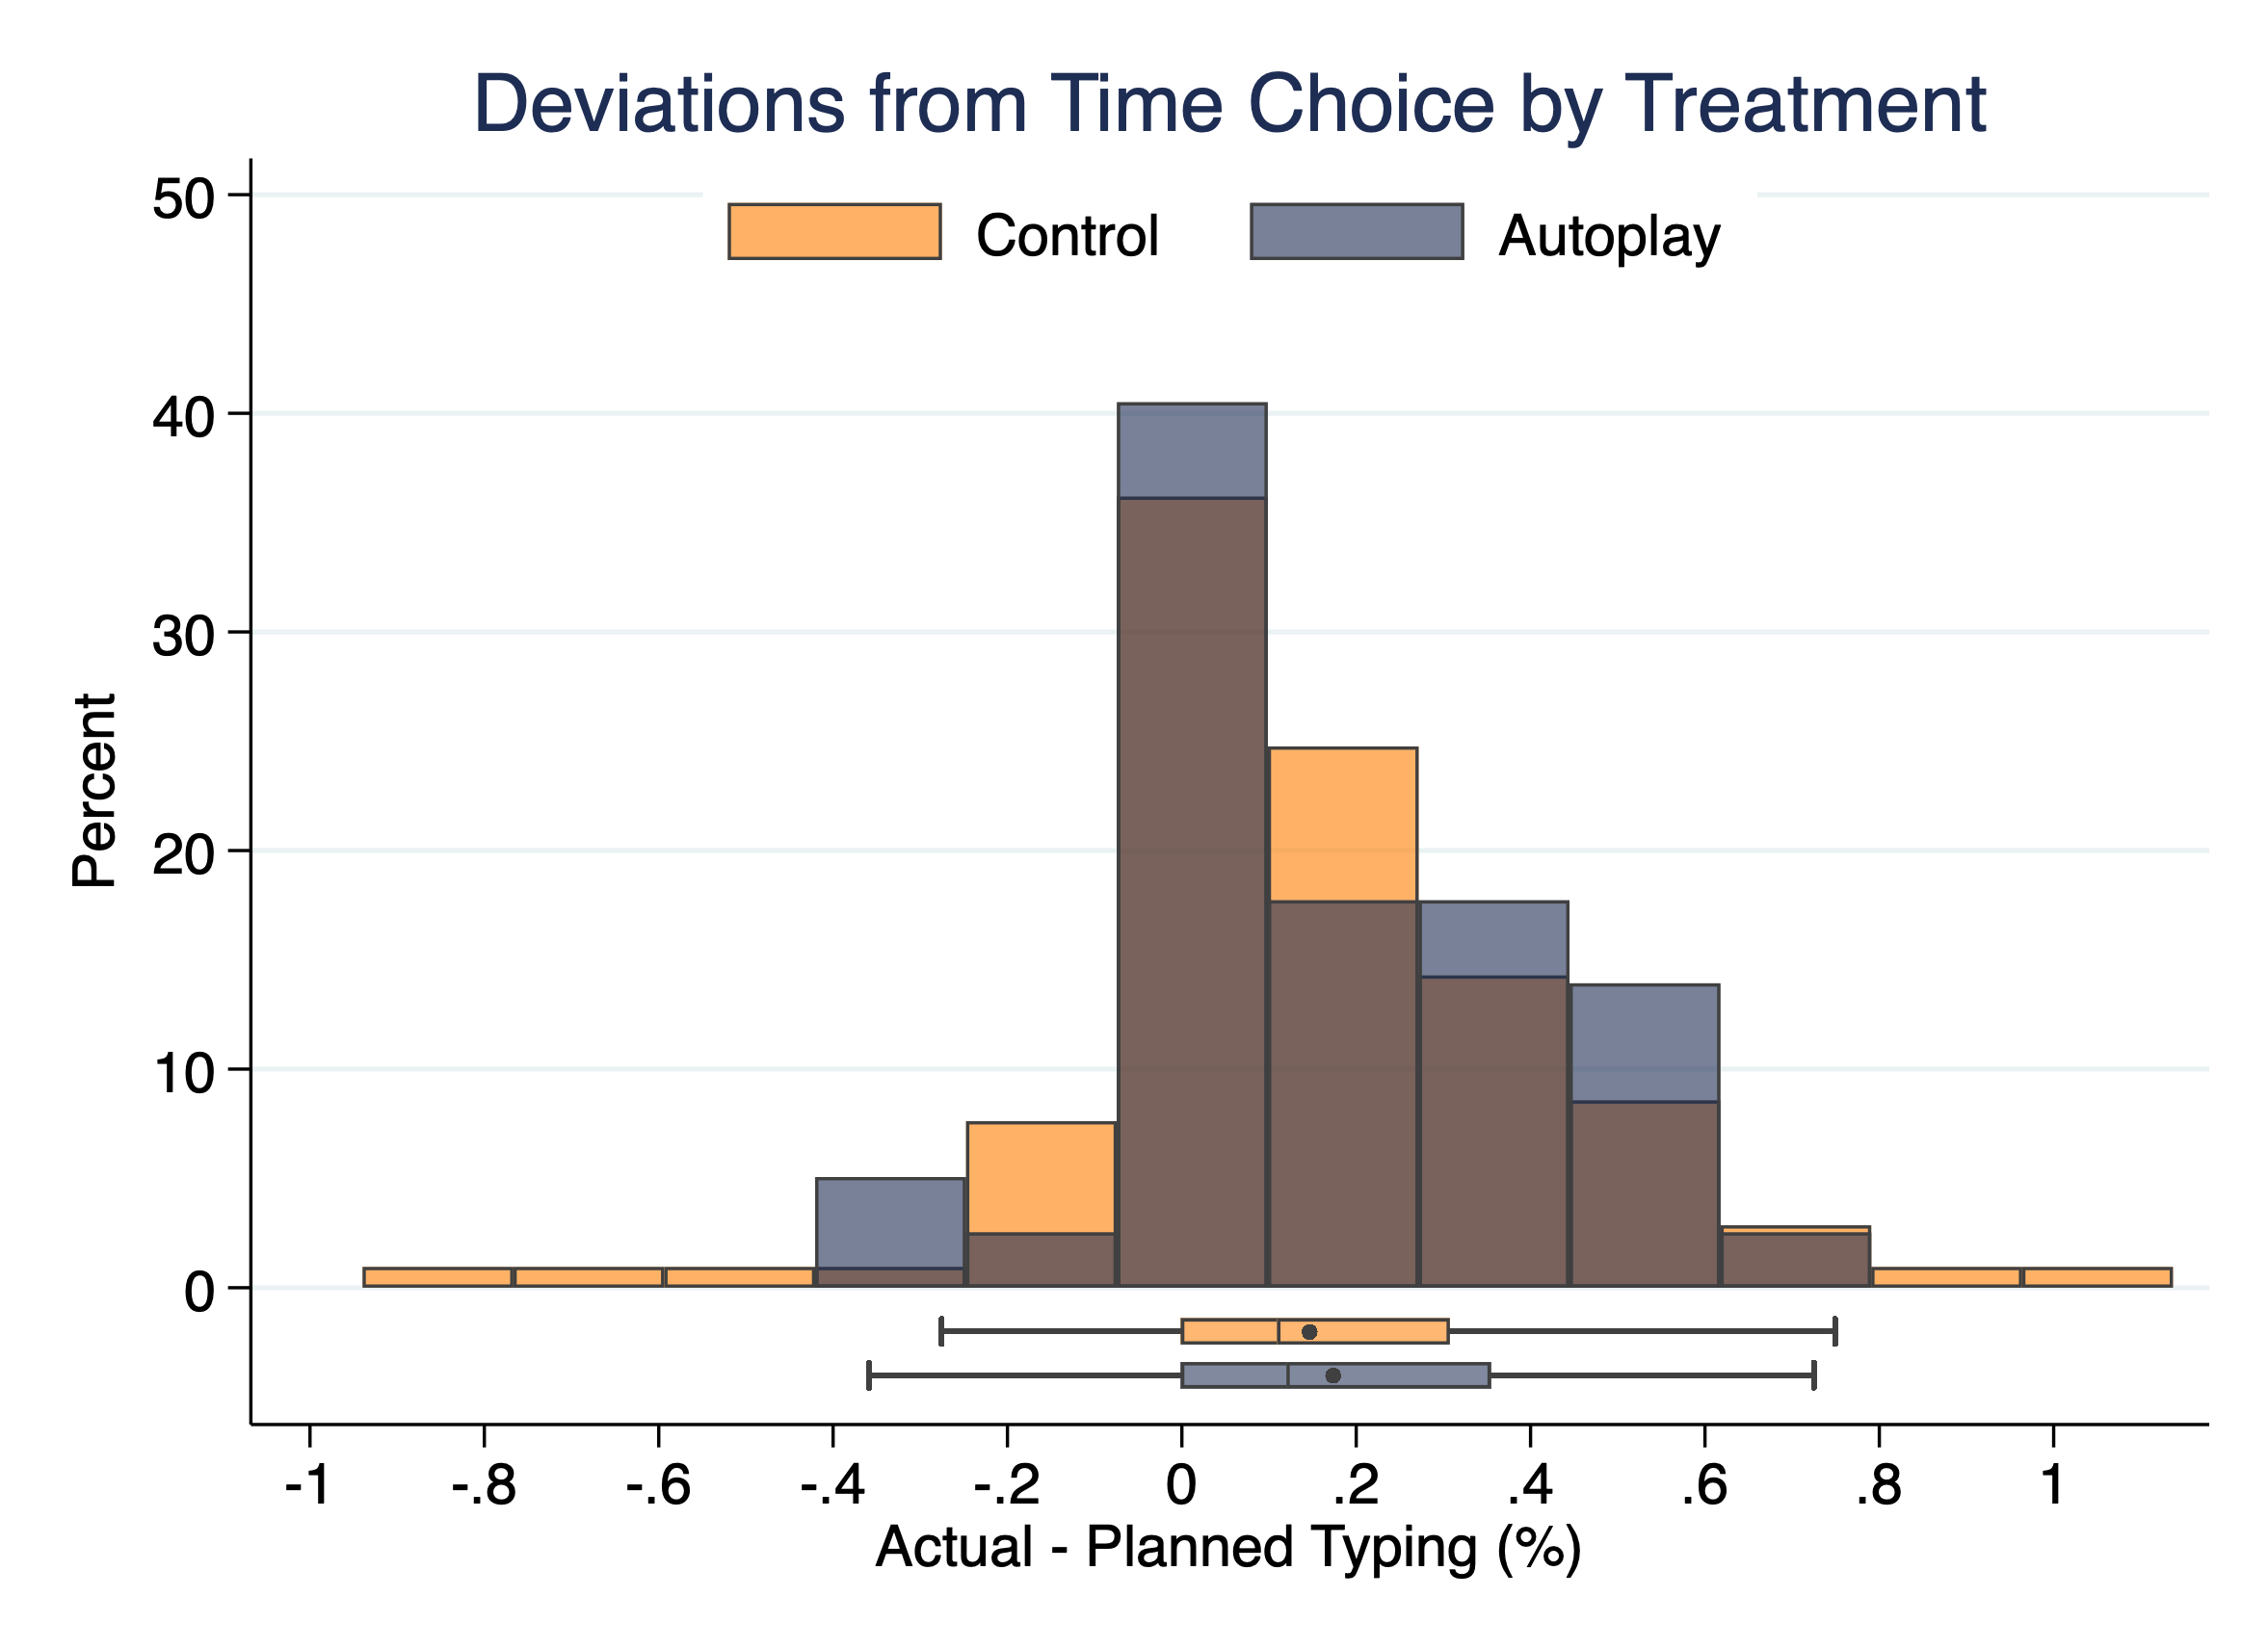
\includegraphics[width=0.9\columnwidth]{deviation_hist.png}
    \end{column}
  \end{columns}
\end{frame}

\begin{frame}{H3: Commitment against autoplay}
  \textbf{Hypothesis 3:} There is positive demand for a commitment device against autoplay.
  \begin{equation}\label{eq2}
    {Y}_{ij} = \beta_{0} + \beta_{1} \text{Bonus}_{ij} + \epsilon_{ij}
  \end{equation}
  \begin{itemize}
    \item where ${Y}_{ij}$ is the binary choice of taking autoplay given the bonus $j$ from the MPL for individual $i$
    \item WTP for autoplay as the sample-averaged effect of bonus $-\beta_{0}/\beta_{1}$
    \item H3 posits $-\beta_{0}/\beta_{1} > 0$ for preference against autoplay
  \end{itemize}
\end{frame}

\begin{frame}{H3: Commitment against autoplay}
  \begin{columns}[T]
    \begin{column}{0.43\textwidth}
      \begin{itemize} %[<+->]
        \item WTP for autoplay is the negative ratio of the constant to the bonus coefficient: $-0.6263/27.9729 = -0.0224$ pounds, or 2.24 pence for the 20-minute session
        \item Participants value autoplay at 6.72 pence/hour and would be willing to forgo this amount to maintain access to the feature
      \end{itemize}
    \end{column}
    \begin{column}{0.52\textwidth}
      \begin{table}
        \centering
        \footnotesize  % Make the entire table smaller
        \begin{threeparttable}
          \begin{tabular*}{\columnwidth}{@{\extracolsep{\fill}}lc}
            \toprule
            & Autoplay\\
            \cmidrule(lr){2-2}
            & (1) \\
            \midrule
            Bonus (£) & 27.973*** \\
            & (6.277) \\
            Constant & 0.626** \\
            & (0.199) \\
            \midrule
            Obs. & 468 \\
            Clusters & 52 \\
            Pseudo $R^2$ & 0.658 \\
            Wald $\chi^2$(1) & 19.86 \\
            \bottomrule
          \end{tabular*}
          \begin{tablenotes}[flushleft]
            \footnotesize
            \tiny
            \item[] \textit{Note:} Logistic regression with standard errors clustered at the participant level in parentheses. Dependent variable is binary choice of selecting autoplay (1) or turning it off (0). Bonus amounts range from £$-0.5$ to £$0.5$. The pseudo $R^2$ indicates good fit. *** $p<0.001$, ** $p<0.01$, * $p<0.05$.
          \end{tablenotes}
        \end{threeparttable}
        \label{tab:wtp_autoplay}
      \end{table}
    \end{column}
  \end{columns}
\end{frame}

\begin{frame}{Main Findings Recap}
  \begin{itemize}
    \item Autoplay did not increase the nb. of video content consumed nor caused more preference reversals (H1 \& H2)
    \item Participants actually deviated from their time allocation plans toward more Transcription!
    \item Participants are willing to pay for the Autoplay feature (H3)
  \end{itemize}
\end{frame}

\begin{frame}{Mechanisms}
  \begin{columns}[T]
    \begin{column}{0.43\textwidth}
      \begin{itemize} %[<+->]
        \item Time inconsistent behavior toward more earnings (max. 60 pence) on Day 2
        \item Why exert more effort than initially planned for?
      \end{itemize}
    \end{column}
    \begin{column}{0.52\textwidth}
      \centering
      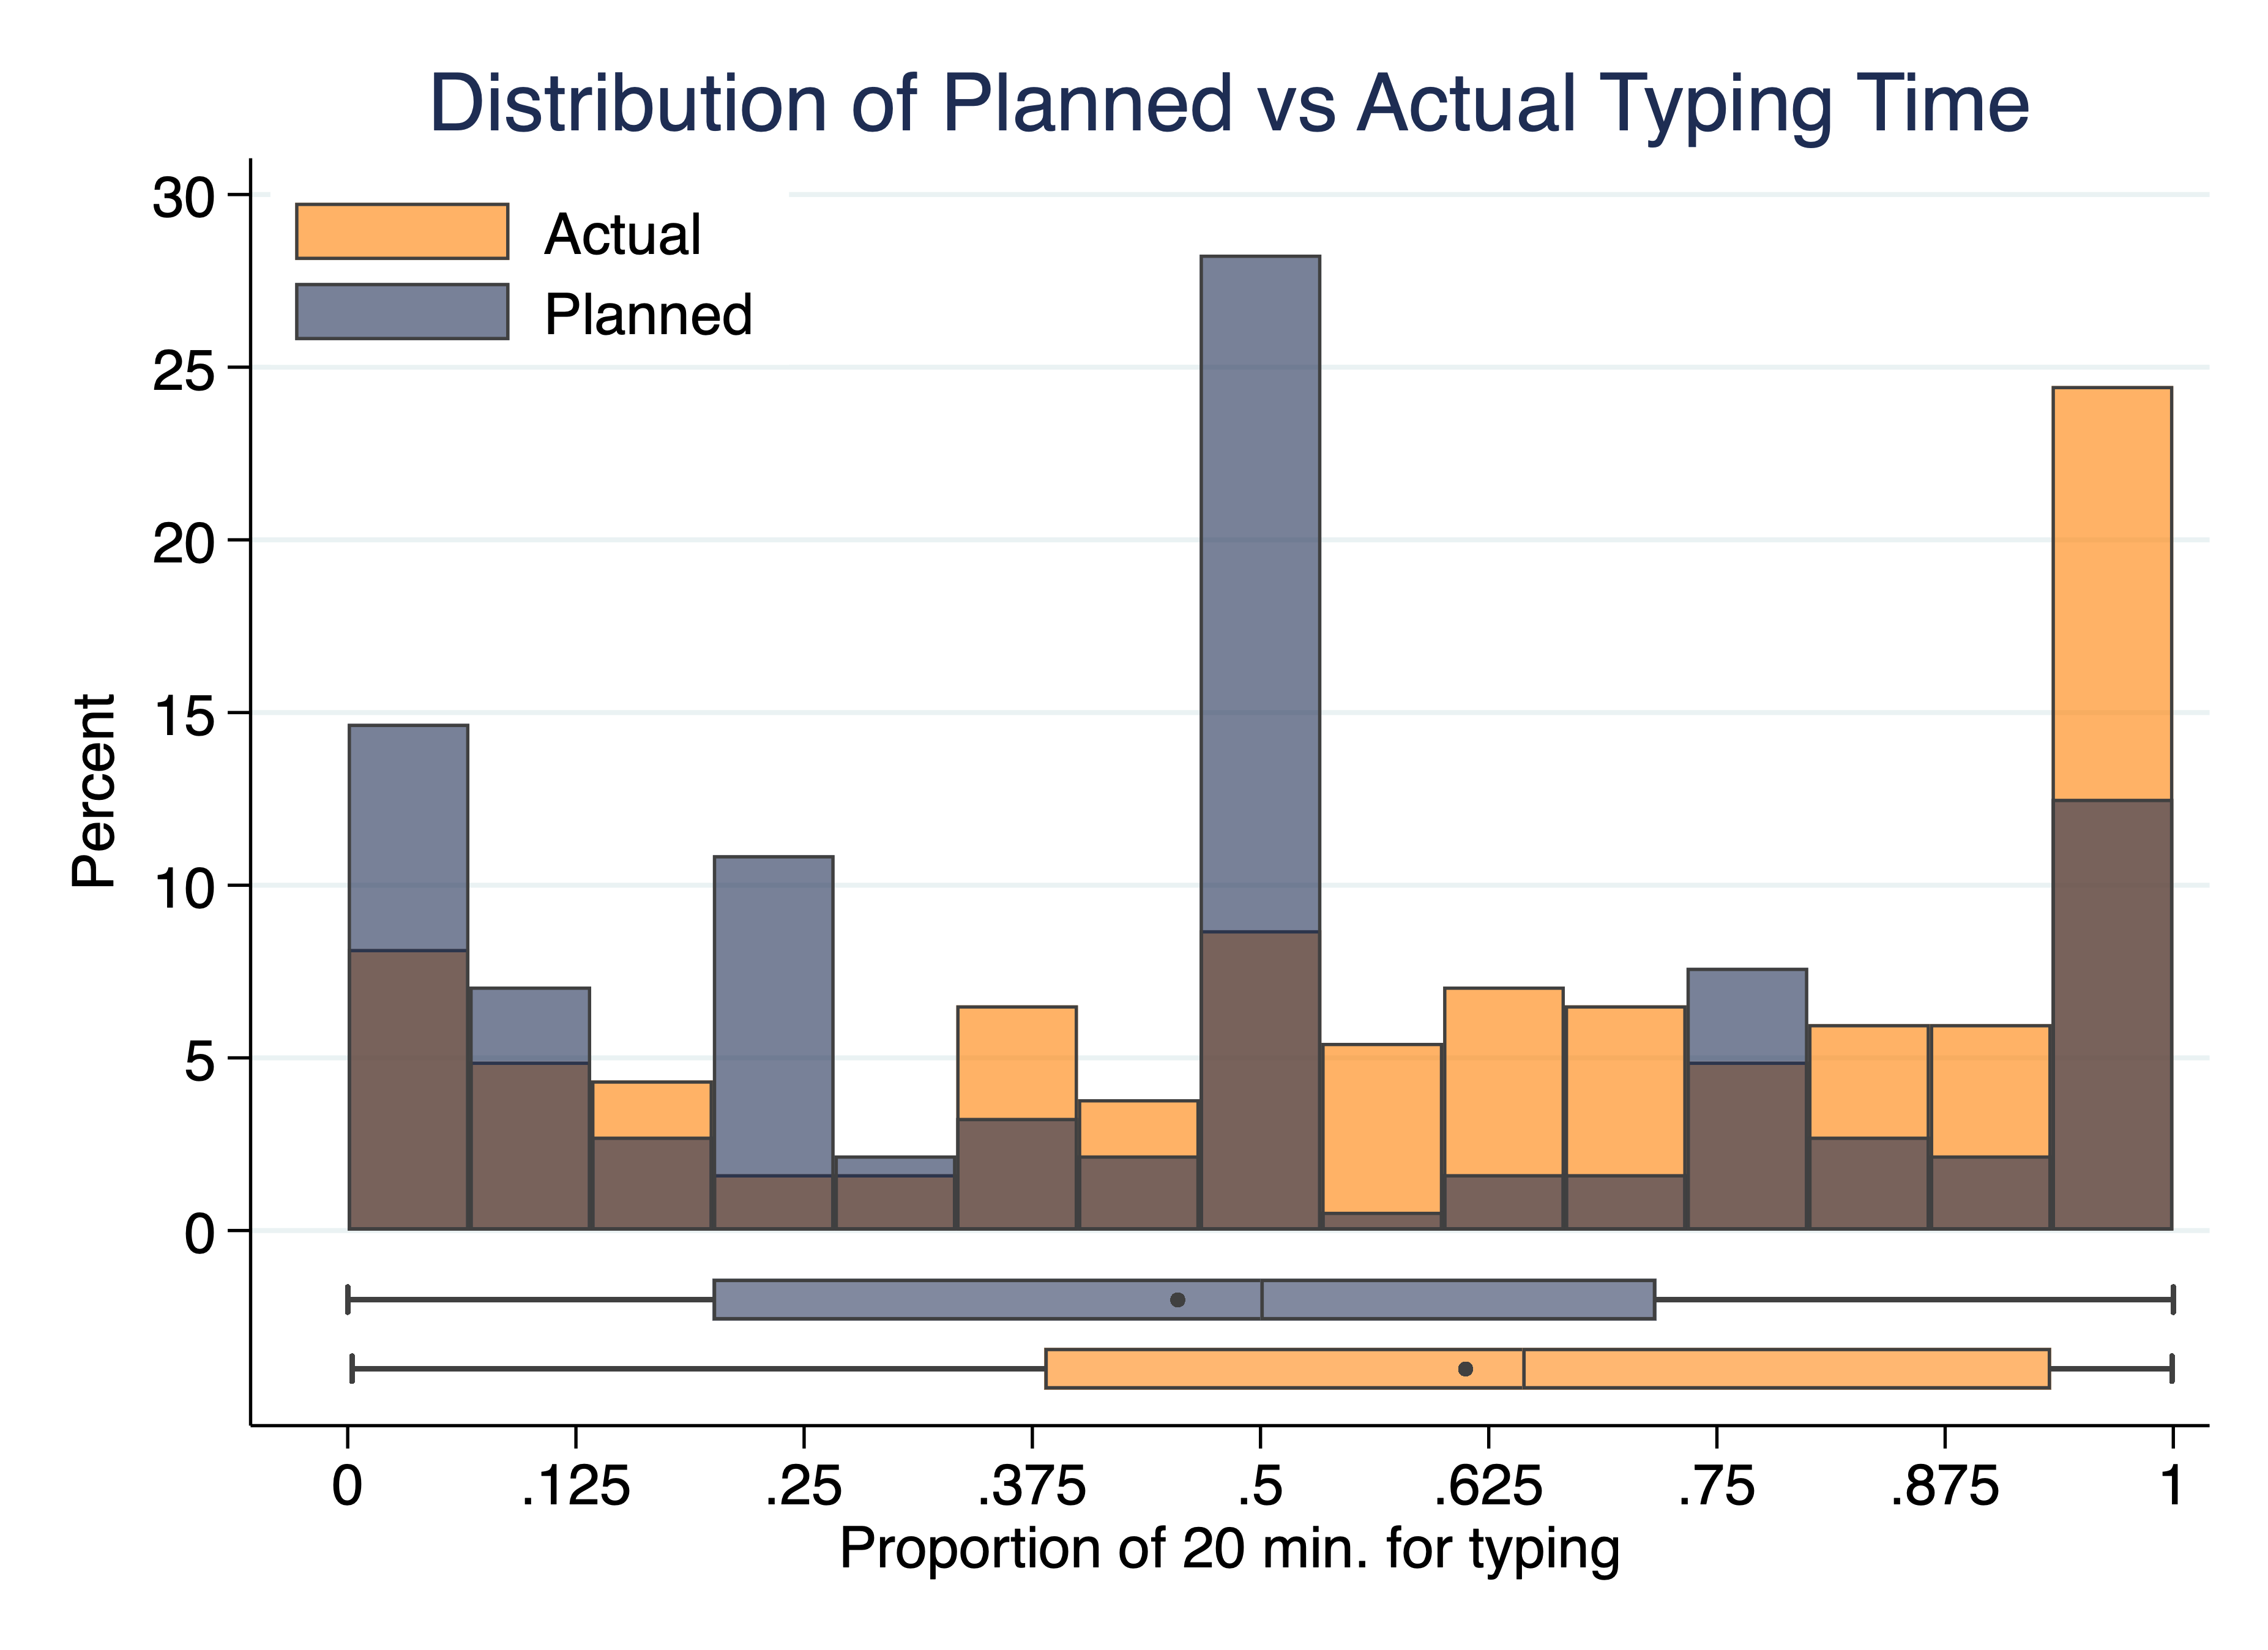
\includegraphics[width=0.9\columnwidth]{dual_typechoice_hist.png}
    \end{column}
  \end{columns}
\end{frame}

\begin{frame}{Free form text analysis}
  \begin{columns}[T]
    \begin{column}{0.49\textwidth}
      \centering
      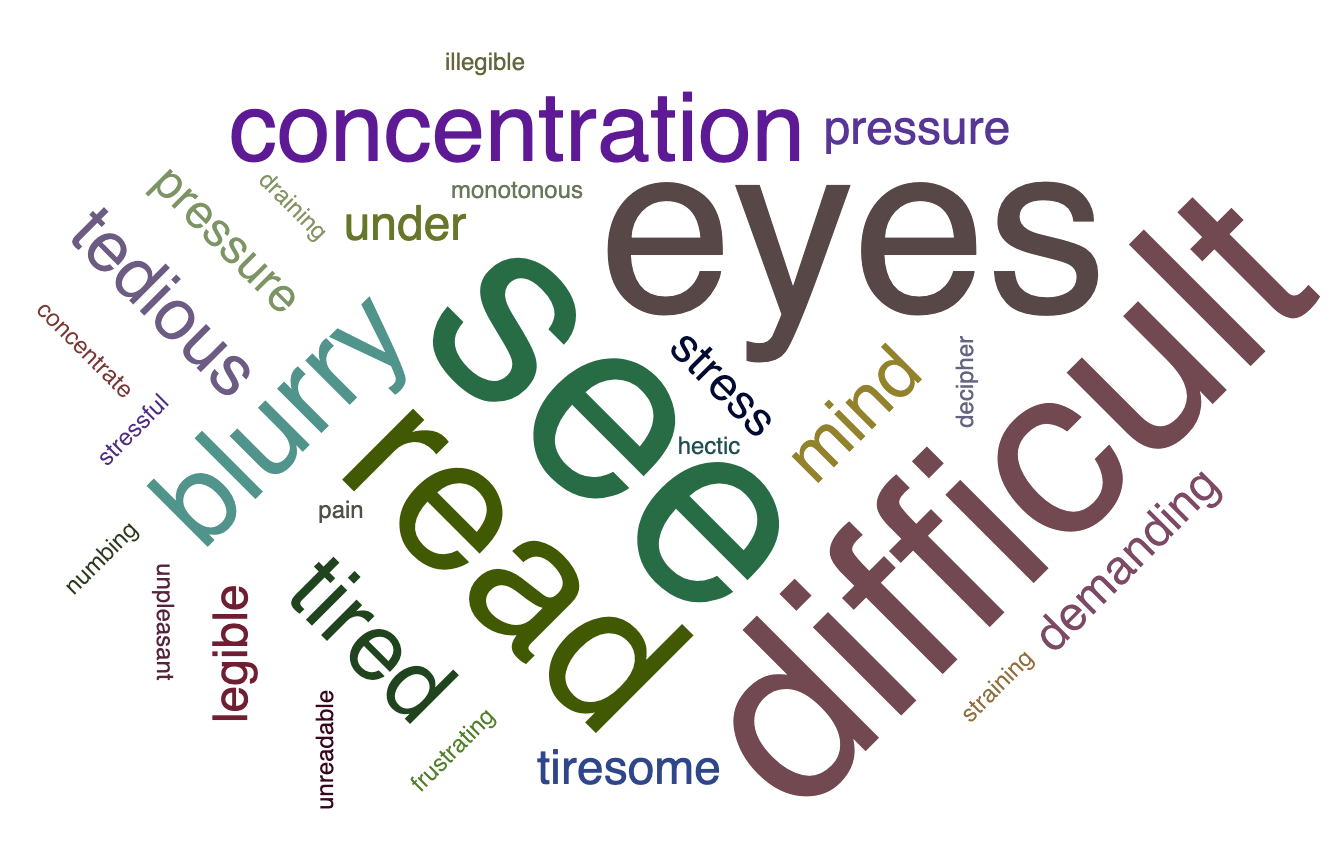
\includegraphics[width=.7\linewidth]{type.png}
    \end{column}
    \begin{column}{0.49\textwidth}
      \centering
      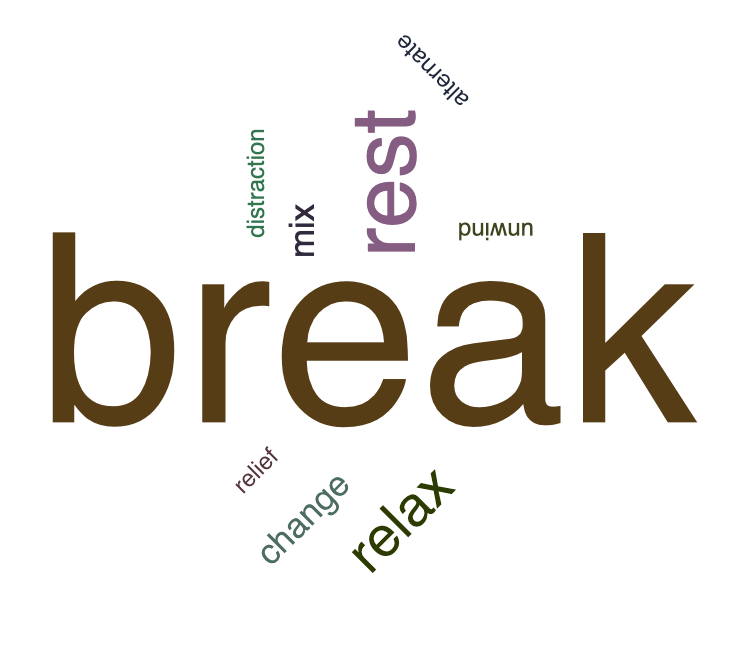
\includegraphics[width=.7\linewidth]{break.png}
    \end{column}
  \end{columns}
  \begin{itemize}
    \item Transcription task was perceived negatively (29\%)
    \item Watching videos as taking breaks from transcription (23\%)
    \item Unintentional ``work environment'' due to experimenter demand effects
  \end{itemize}
\end{frame}

\begin{frame}{Achieving Time Allocation Plans}
  \begin{columns}[T]
    \begin{column}{0.38\textwidth}
      \begin{itemize} %[<+->]
        \item Regression Discontinuity with 30-second bins around planned time allocation
        \item Participants aim to achieve their plans...
        \item ...but eventually they get back to ``work''
      \end{itemize}
    \end{column}
    \begin{column}{0.62\textwidth}
      \centering
      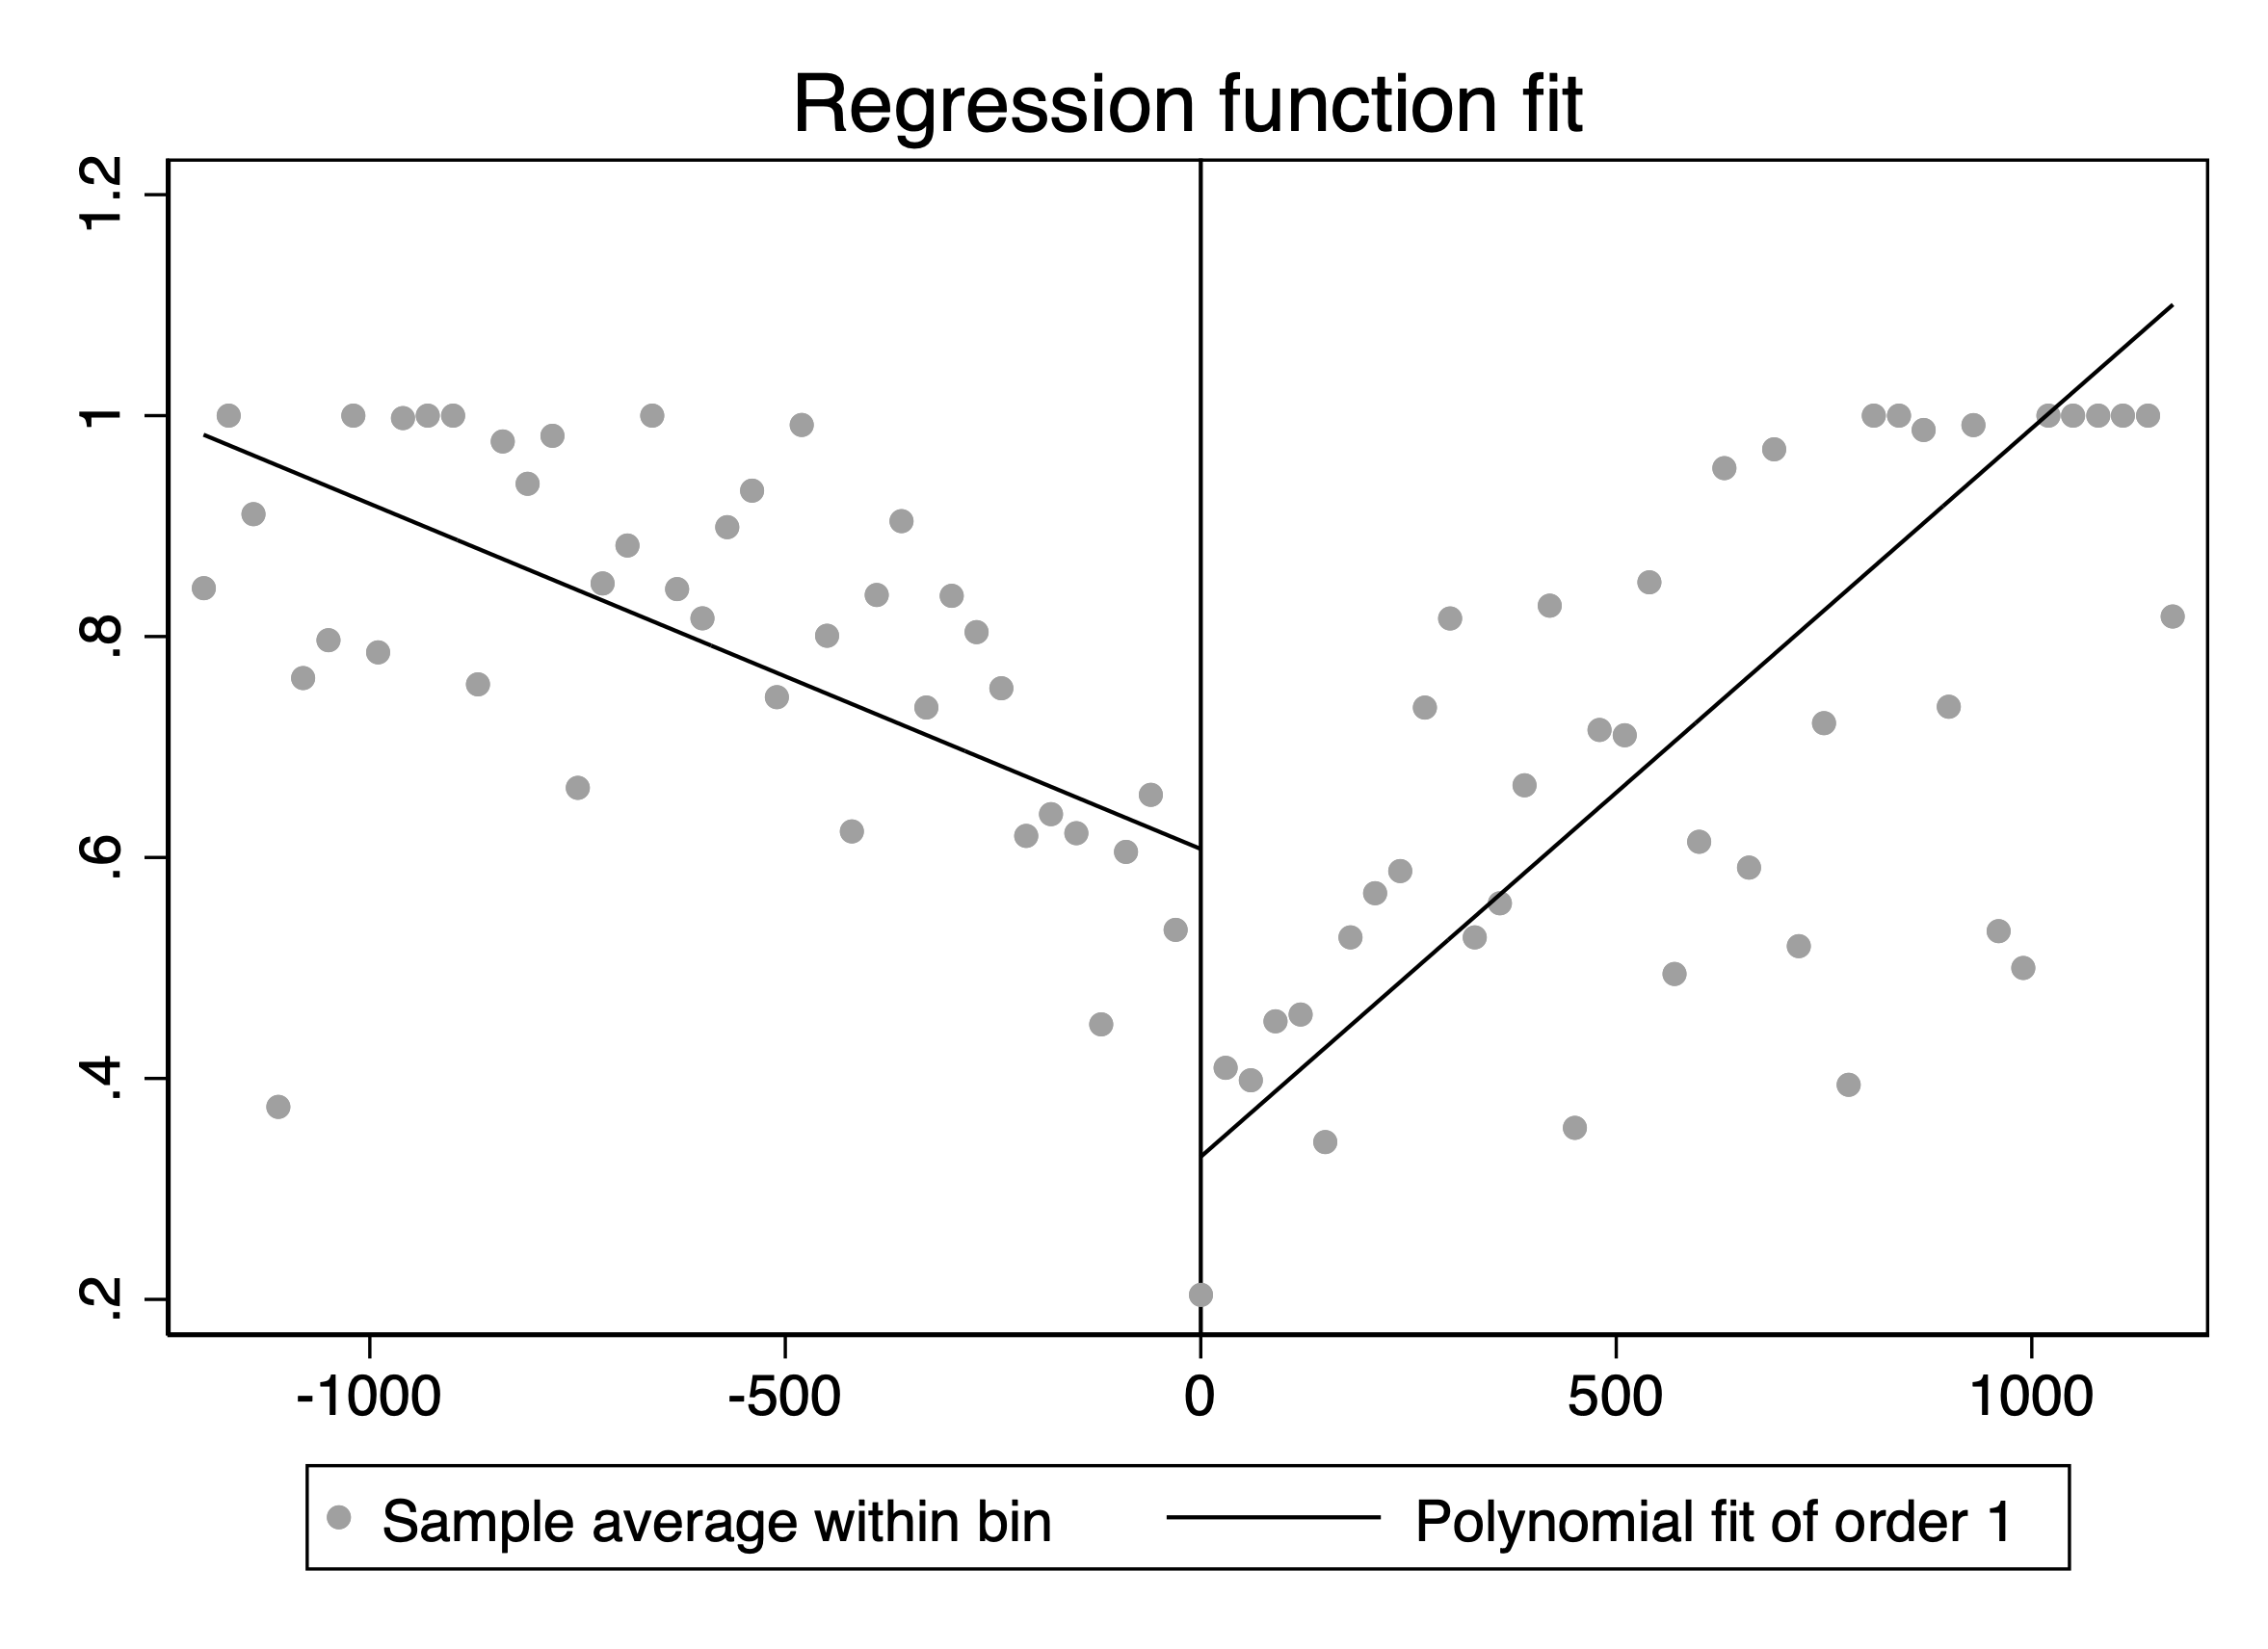
\includegraphics[width=0.9\columnwidth]{rd_bin30.png}
    \end{column}
  \end{columns}
\end{frame}

\begin{frame}{Conclusion}
  \begin{itemize} %[<+->]
    \item First study to causally identify autoplay's effect on content consumption
    \item Methodological: unexpected within the intertemporal choice framework (implementation)
    \item Causes: study design (earnings difference, focus on transcription requirements), quirks of the Prolific participant pool (research for a living), postponing leisure after the experiment (spoonfeeding leisure)
    \item Policy: more suitable for field work, albeit more intruisive and technically complex
  \end{itemize}
\end{frame}

\begin{frame}{Why pay for Autoplay?}
  \hideprogressbar
  \begin{table}
    \centering
    \begin{threeparttable}
      \begin{tabular*}{0.8\textwidth}{@{\extracolsep{\fill}}lccc}
        \toprule
        & Control & Autoplay & Difference \\
        \midrule
        Total seconds lost & 46.52 & 1.08 & 45.45*** \\
        & (9.27) & (0.65) & (9.29) \\
        \midrule
        Observations & 105 & 79 & 184 \\
        $t$-statistic & & & 4.89 \\
        \bottomrule
      \end{tabular*}
    \end{threeparttable}
  \end{table}
  \begin{itemize} %[<+->]
    \item Efficiency gains
    \item Easing consumption
  \end{itemize}
\end{frame}

\begin{frame}{Robustness: Participant Behavior}
  \begin{columns}[T]
    \begin{column}{0.45\textwidth}
      \centering
      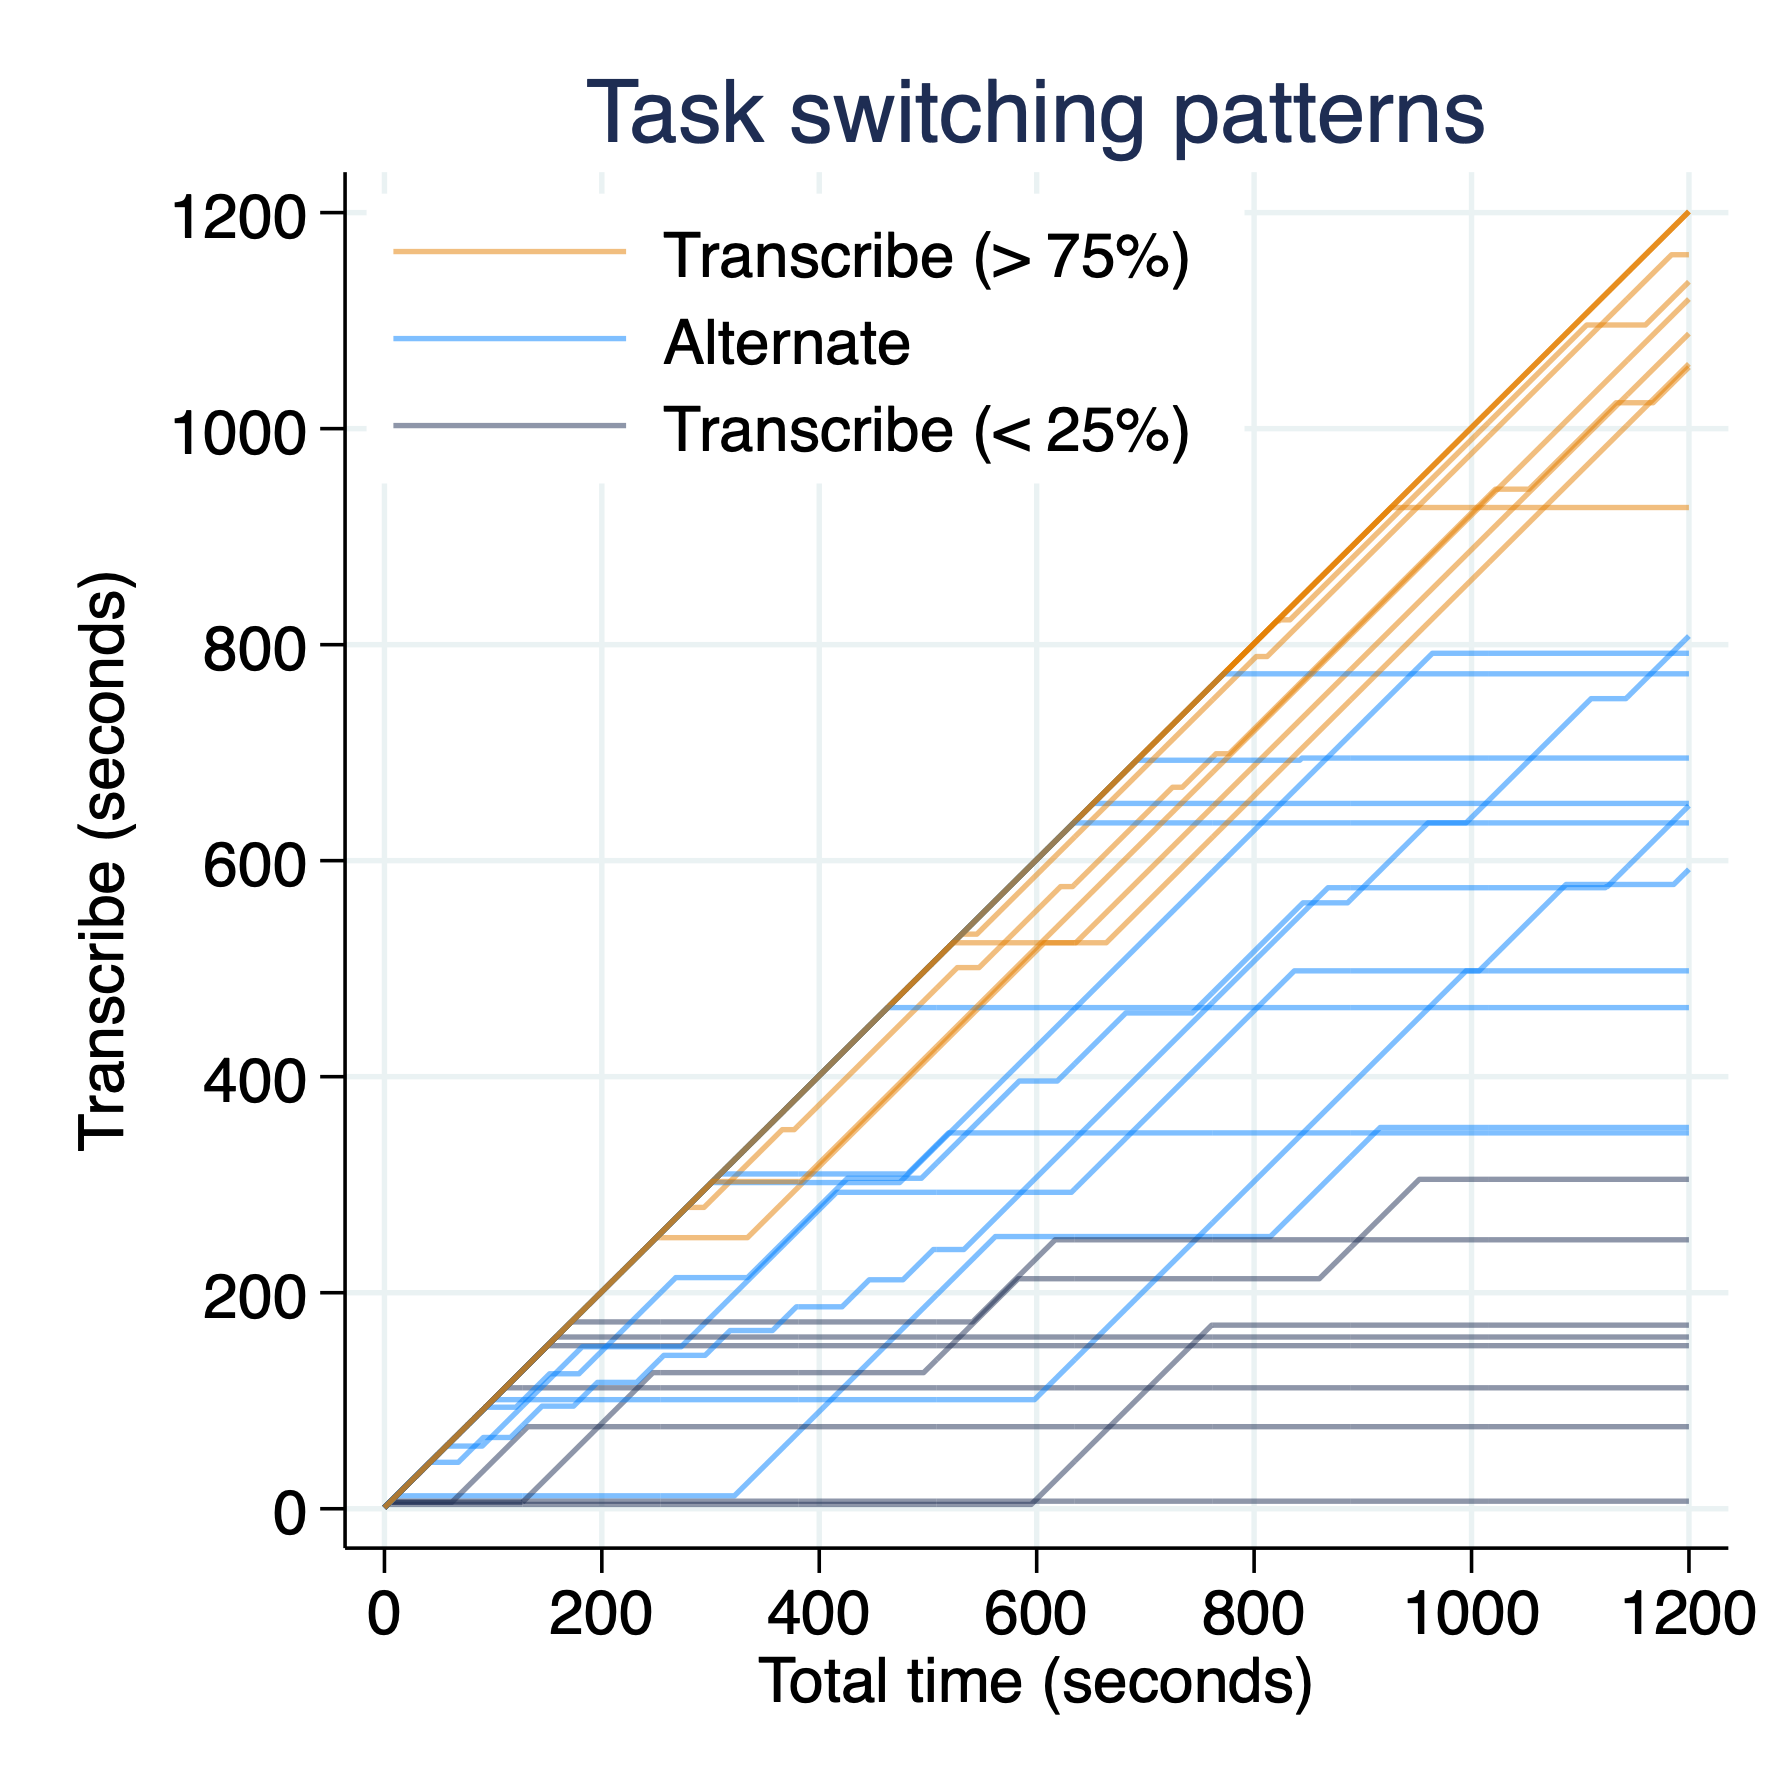
\includegraphics[width=0.9\columnwidth]{typing_cdf.png}
    \end{column}
    \begin{column}{0.45\textwidth}
      \centering
      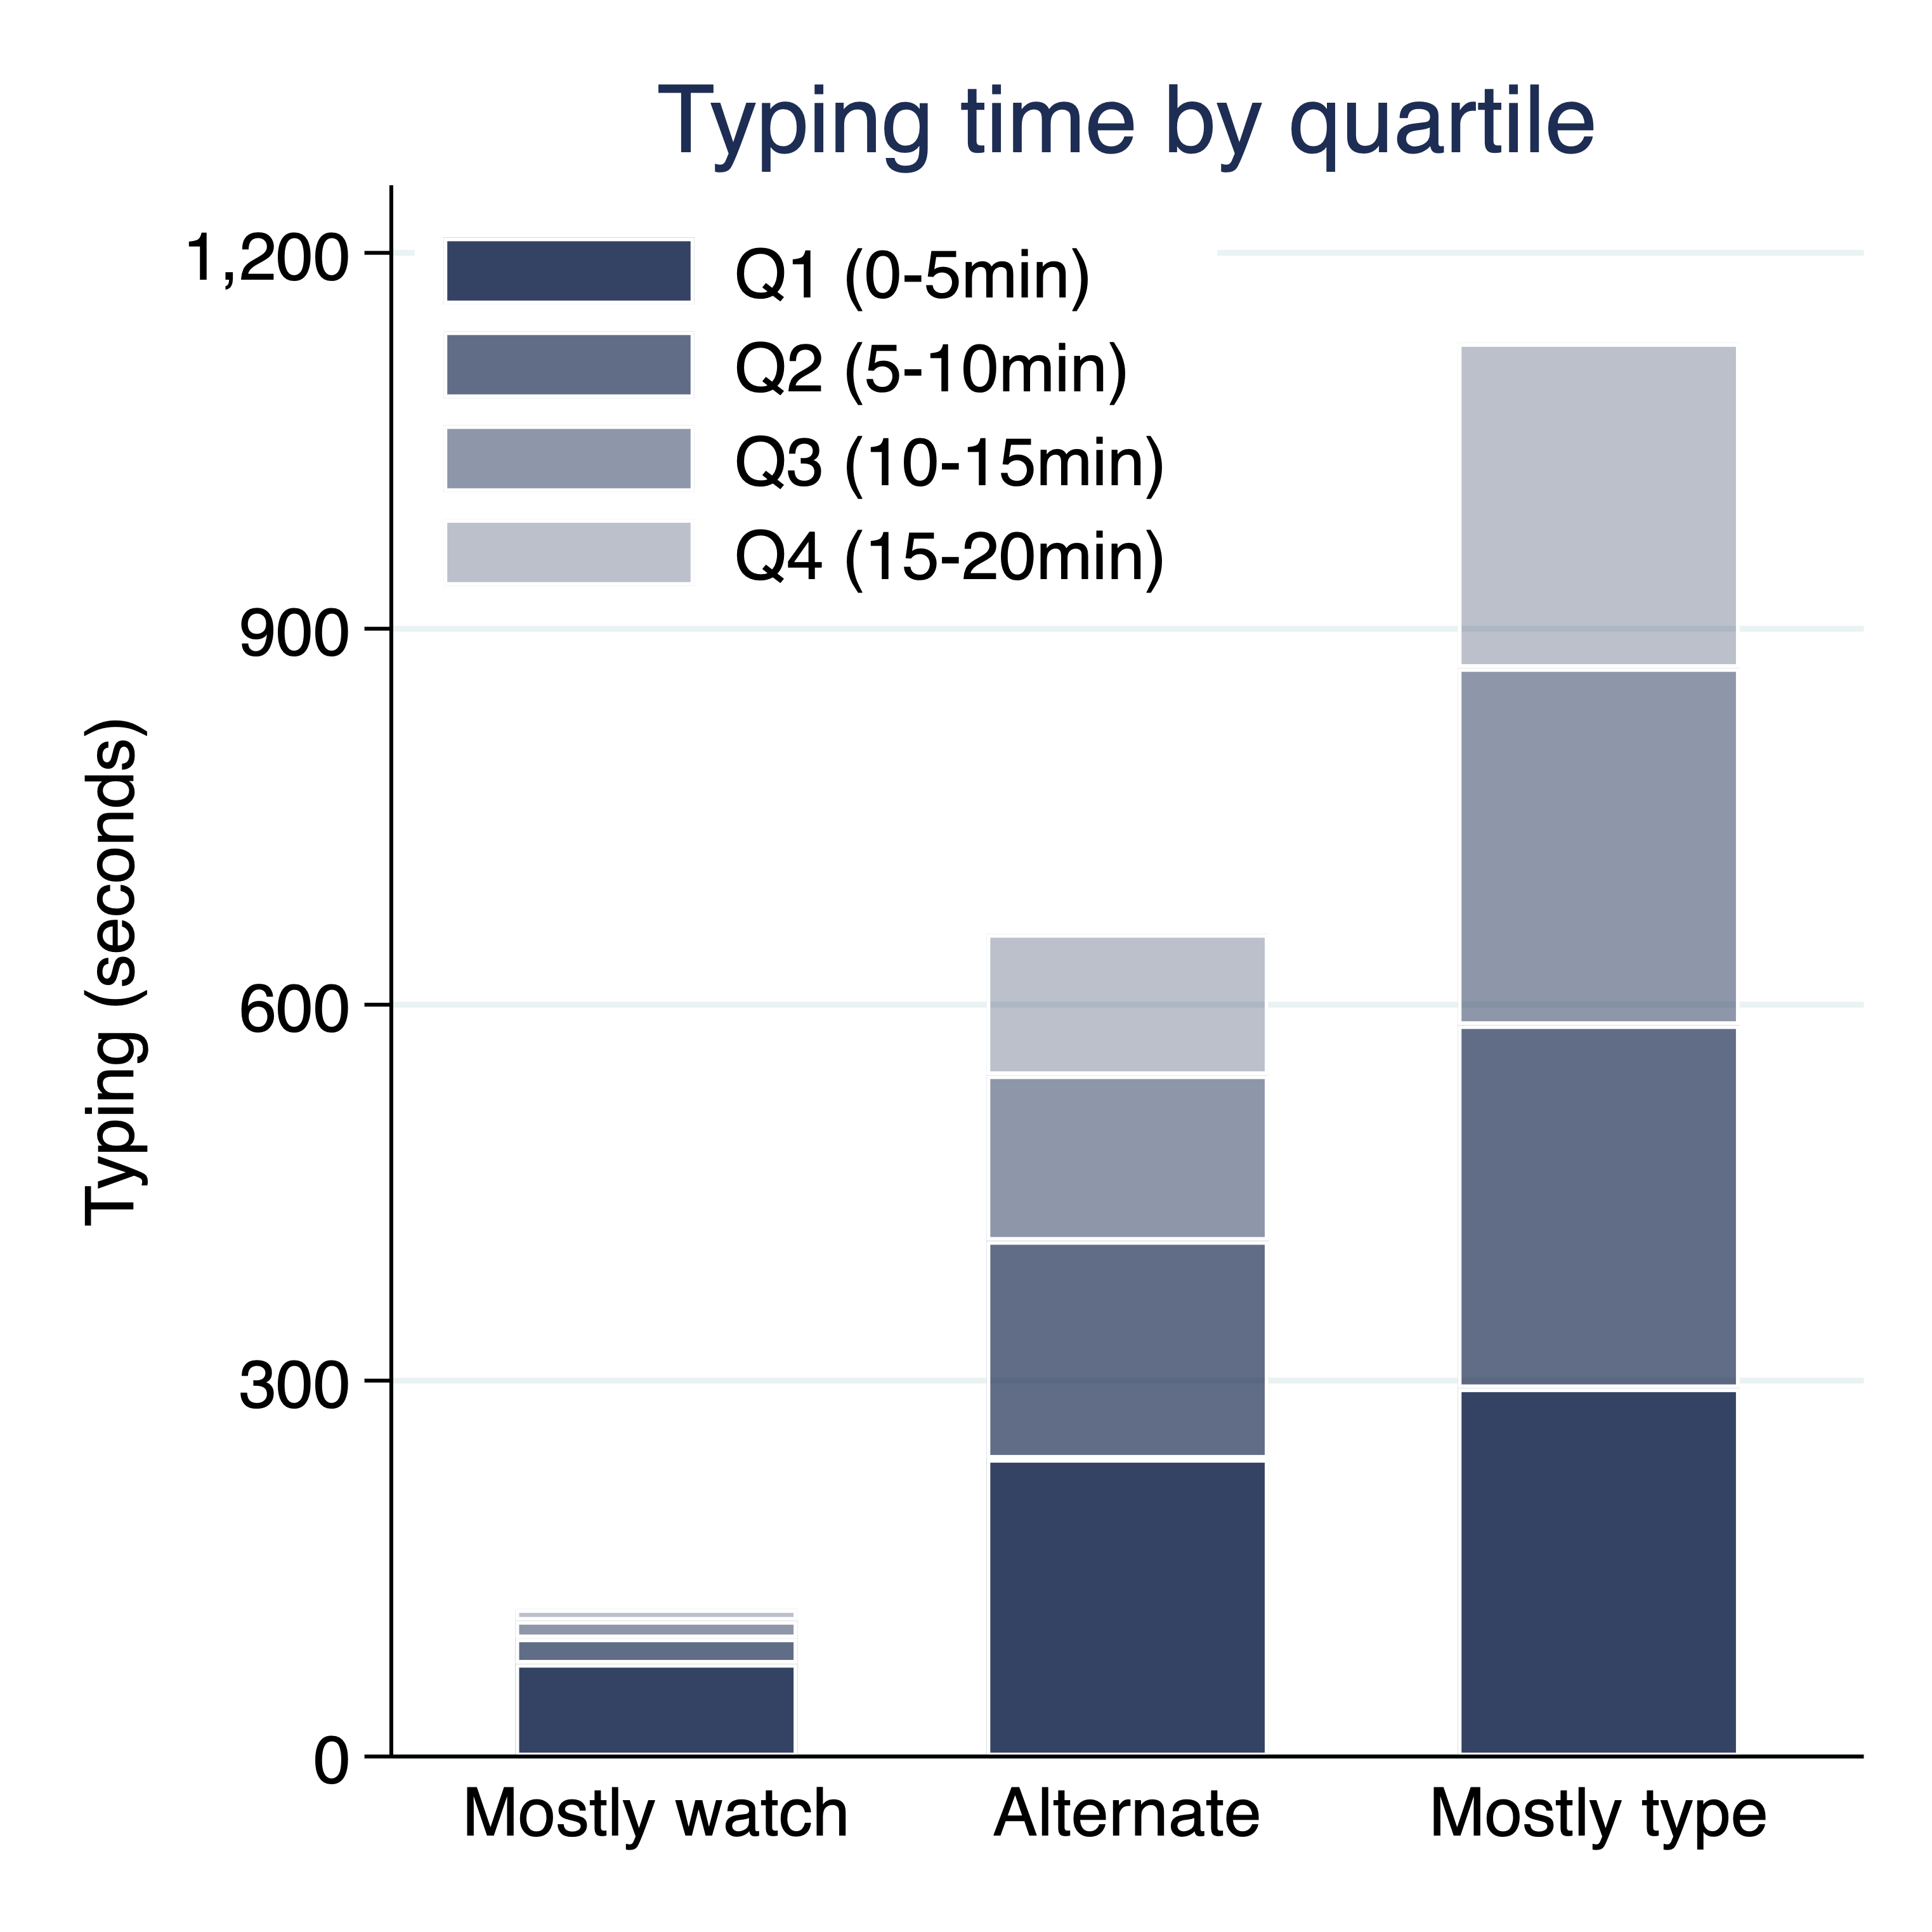
\includegraphics[width=0.9\columnwidth]{work_allocation_quartiles.png}
    \end{column}
  \end{columns}
\end{frame}

\begin{frame}{Robustness: Full Sample}
  \begin{table}
    \footnotesize
    \centering
    \begin{threeparttable}
      \begin{tabular*}{0.9\textwidth}{@{\extracolsep{\fill}}lccc}
        \toprule
        & \multicolumn{3}{c}{Nb. of Videos Watched (z-score)} \\
        \cmidrule(lr){2-4}
        & (1) & (2) & (3) \\
        \midrule
        Autoplay & 0.051 & 0.131 & 0.132 \\
        & (0.135) & (0.109) & (0.109) \\
        Time Choice (z-score) & & $-$0.590*** & $-$0.555*** \\
        & & (0.060) & (0.084) \\
        Autoplay × Time Choice & & & $-$0.077 \\
        & & & (0.118) \\
        Constant & $-$0.023 & $-$0.061 & $-$0.059 \\
        & (0.090) & (0.075) & (0.075) \\
        \midrule
        Obs. & 224 & 224 & 224 \\
        $R^2$ & 0.001 & 0.347 & 0.348 \\
        $F$-statistic & 0.14 & 48.91 & 34.21 \\
        \bottomrule
      \end{tabular*}
      \begin{tablenotes}[flushleft]
        \footnotesize
        \item[] \textit{Note:} Robust standard errors in parentheses. All variables are standardized. Time Choice represents participants' planned typing proportion from day 1. *** $p<0.001$, ** $p<0.01$, * $p<0.05$.
      \end{tablenotes}
    \end{threeparttable}
  \end{table}
\end{frame}

\begin{frame}{Full RD table}
  \begin{table}
    \footnotesize
    \centering
    \begin{threeparttable}
      \begin{tabular*}{0.8\textwidth}{@{\extracolsep{\fill}}lccc}
        \toprule
        & \multicolumn{3}{c}{Time Window} \\
        \cmidrule(lr){2-4}
        & 30-seconds & 60-seconds & 90-seconds \\
        \midrule
        Proportion transcribing & -0.274*** & -0.255*** & -0.075 \\
        & (0.101) & (0.087) & (0.108) \\
        \midrule
        Obs. (left) & 66,786 & 67,985 & 67,119 \\
        Obs. (right) & 80,270 & 89,006 & 92,999 \\
        Clusters (left) & 157 & 154 & 155 \\
        Clusters (right) & 154 & 157 & 161 \\
        Bandwidth & 339.9 & 368.3 & 422.3 \\
        \bottomrule
      \end{tabular*}
    \end{threeparttable}
  \end{table}
\end{frame}

\begin{frame}[allowframebreaks]{References}
  \bibliographystyle{apacite}
  \bibliography{references}
\end{frame}

\end{document}

% \begin{itemize}
%   \item 
%   \item Balanced demographics across conditions

%   \item Session duration: <30 min across 2 days
% \end{itemize}
